\section*{\fontsize{16}{14}\selectfont Aim: Getting  familiar and hands on practice with testing tools like win runner, selenium etc.}
Software Testing Tools in the market. Selection of tools is totally based on the project requirements \& commercial (Proprietary/Commercial tools) or free tools (Open Source Tools) you are interested. Off Course, free Testing Tools may have some limitation in the features list of the product, so it’s totally based on what are you looking for \& is that your requirement fulfill in free version or go for paid Software Testing Tools.
The following tools can be used for automation testing:
\begin{enumerate}
\item \textbf{HP Quick Test Professional:}
HP QuickTest Professional was renamed to HPE Unified Functional Testing. HPE UFT offers testing automation for functional and regression testing for the software applications.Visual Basic Scripting Edition scripting language is used by this tool to register the  test processes and operates the various objects and controls in testing the applications.
QTP offers various features like:
\begin{itemize}
\item Integration with Mercury Business Process Testing and Mercury Quality Center
\item Unique Smart Object Recognition
\item Error handling mechanism
\item Creation of parameters for objects, checkpoints, and data-driven tables
\item Automated documentation
\end{itemize}
\item \textbf{Selenium:}
Selenium is a testing framework to perform web application testing across various browsers and platforms like Windows, Mac, and Linux. Selenium helps the testers to write tests in various programming languages like Java, PHP, C\#, Python, Groovy, Ruby, and Perl. It offers record and playback features to write tests without learning Selenium IDE.
Selenium proudly supports some of the largest, yet well-known browser vendors who make sure they have Selenium as a native part of their browser. Selenium is undoubtedly the base for most of the other software testing tools in general.

\item \textbf{TestComplete:}
TestComplete is a functional testing platform that offers various solutions to automate testing for desktop, web, and mobile applications by SmartBear Software.
TestComplete offers the following features:
\begin{itemize}
\item GUI testing
\item Scripting Language Support: JavaScript, Python, VBScript, JScript, DelphiScript, C++Script \& C\#Script
\end{itemize}

\item \textbf{WinRunner:}
WinRunner is a program that is responsible for the automated testing of software. It is designed to function with Windows applications, and it was designed by Mercury Interactive Corporation, an organization that is based in California. WinRunner will allow you to make comparisons between various outcomes. 
A series of wizards will be provided to the user, and these wizards can create tests in an automated manner. Another impressive aspect of Winrunner is the ability to record various interactions, and transform them into scripts. WinRunner is designed for testing GUIs, or Graphic User Interfaces.
When the user make an interaction with the GUI, this interaction can be recorded. Recording the interactions will allow you to determine various bugs that need to be fixed. The goal of WinRunner is to make sure business processes are properly carried out. WinRunner uses TSL, or Test Script Language. The input of the user can be customized at various levels. WinRunner will test the computer program in a way that is very similar to normal user interactions. This is important, because it ensures a high level of accuracy and realism. Even if an engineer is not physically present, the Recover manager will troubleshoot any problems that may occur, and this will allow the tests to be completed without errors


\item \textbf{WATIR:}
Watir is an open source testing tool made up of Ruby libraries to automate web application testing. It is pronounced as "water."
Watir offers following features:
\begin{itemize}
\item Tests any language-based web application
\item Cross-browser testing
\item Compatible with business-driven development tools like RSpec, Cucumber, and Test/Unit
\item Tests web page's buttons, forms, links, and their responses
\end{itemize}

\textbf{Tools Implementation - process}
\begin{enumerate}
\item Analyse the problem carefully to identify strengths, weaknesses and opportunities 
\item The Constraints such as budgets, time and other requirements are noted.
\item Evaluating the options and Shortlisting the ones that are meets the requirement
\item Developing the Proof of Concept which captures the pros and cons
\item Create a Pilot Project using the selected tool within a specified team
\item Rolling out the tool phase wise across the organization
\end{enumerate}
\end{enumerate}
\textbf{Installation of Selenium}\\
Installation of Selenium is a very easy process.
The current git version is: 3.4.0.
Type the commands in the terminal:\\\\
\emph{
\$ sudo apt-get update\\\\
\$ sudo apt-get install pip3\\\\
\$ pip3 install selenium\\\\}
This will install the selenium on your pc or laptop.\\\\
\textbf{Testing of the project using selenium}\\
The webdriver for Firefox is installed along with Selenium but if you want to test your applications on chrome then you need to download the chrome driver and ensure chrome is installed on your Linux distro.\\
\textbf{sel.py file}\\\\
\#!/usr/bin/env python3\\
from selenium import webdriver\\
driver = webdriver.Chrome("/home/amisha/Downloads/chromedriver")\\
driver.get("http://localhost/Certificate/CGS/index.php?cert=design4")\\
assert "Academic Certificate" in driver.title\\
innn=driver.find\_element\_by\_name("in")\\
innn.send\_keys("Selenium web test edit")\\
asss=driver.find\_element\_by\_name("as")\\
asss.send\_keys("Selenium web test edit")\\
Submit=driver.find\_element\_by\_value("Submit")\\
success=Submit.click()\\
assert "Institute Details Saved Succesfully!" in driver.h2\\\\
It is the python script which is used to test the page in the project.
\begin{figure}[!ht]
\centering
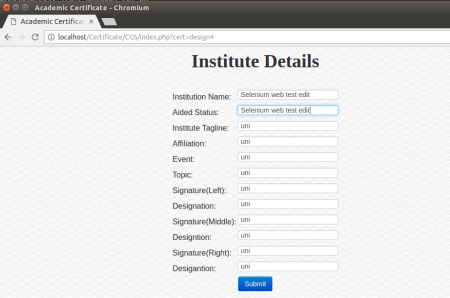
\includegraphics[width=0.8\linewidth]{input/images/se3.png}
\label{fig:image1}
\caption{Testing Automatically}
\end{figure}
\begin{figure}[!ht]
\centering
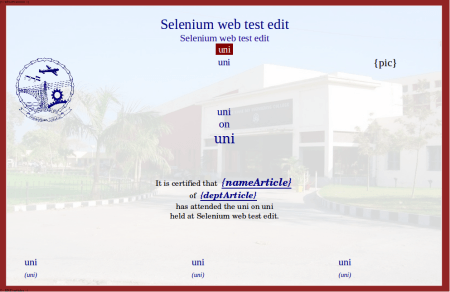
\includegraphics[width=0.8\linewidth]{input/images/se5.png}
\label{fig:image1}
\caption{Certificate Generated}
\end{figure}

